\documentclass[letter,12pt]{article}
%
\input{def}
\usepackage[table]{xcolor}
\usepackage{relsize}
\usepackage{bm}
\usepackage{mathrsfs}
\newcommand{\angstrom}{\mbox{\normalfont\AA}}

 \def\ol{\overline}
 \def\no{\noindent}
 \def\qd{\dot{Q}}
%%%%%%%FLOW DIAGRAM%%%%%%%%%%
\usepackage[latin1]{inputenc}
\usepackage{tikz}
%\usepackage[table]{xcolor}
\usetikzlibrary{shapes,arrows}
% Define block styles
\tikzstyle{decision} = [diamond, draw, fill=blue!20, 
   text width=5.0em, text badly centered, node distance=3cm, inner sep=0pt]
\tikzstyle{block} = [rectangle, draw, fill=cyan!20, 
   text width=9.0em, text centered, rounded corners]
\tikzstyle{line} = [draw, -latex']
\tikzstyle{cloud} = [draw, ellipse,fill=red!20, node distance=3cm,
   minimum height=2em]
%%%%%%%%%%%%%%%%%%%%%%%%%%
%% Algorithm %%%%%
\usepackage[linesnumbered]{algorithm2e}
\newcommand{\nosemic}{\renewcommand{\@endalgocfline}{\relax}}% Drop semi-colon ;
\newcommand{\dosemic}{\renewcommand{\@endalgocfline}{\algocf@endline}}% Reinstate semi-colon ;
\newcommand{\pushline}{\Indp}% Indent
\newcommand{\popline}{\Indm\dosemic}% Undent
\let\oldnl\nl% Store \nl in \oldnl
\newcommand{\nonl}{\renewcommand{\nl}{\let\nl\oldnl}}% Remove line number for one
\SetKwRepeat{Do}{do}{while}
%%%%%%%%%%%%%%%%%

%-------------------------------------------------------------------
\begin{document}

\thispagestyle{empty}
\input{cover}

\baselineskip=22pt

\tableofcontents

\input{abstract}
\clearpage

\section{Introduction}
\label{sec:intro}

\begin{comment}
1. Background on use of MD simulations for thermal transport, preferred for studying
thermal transport by phononic interactions (refer notes from book suggested by Amuthan)


2. One approach to NEMD is the Direct Method, commonly used for estimating the bulk
thermal conductivity. A brief discussion on the direct method and associated pros and cons
(notes from Dellan's paper and book suggested by Amuthan) 
Predictions impacted by the choice of potential, values of
individual parameters, size, and potentially due to duration and applied thermal gradients
(cite Amuthan book, Francesco's paper, McGaughey's paper). 
Errors are introduced by thermostatting (Amuthan book). Nominal value of SW potential parameters based on fitting against experiments and to ensure structural stability etc. (SW paper)

3. Motivate uncertainty analysis and briefly discuss and cite recent efforts (Francesco, Kirby,
Murthy). Highlight focus and key contributions of the present work and how it differs from
those efforts. 

4. Section-wise overview of the paper.  
\end{comment}

Classical Molecular Dynamics (MD) is commonly used to study thermal transport in material systems 
especially in situations where transport due to phonon-phonon interactions is predominant. These 
systems typically comprise non-metallic elements such as carbon (nanotubes, fullerenes, graphite, etc.),
silicon and germanium. 
\bigskip
\bigskip
%
%
\section{NEMD Set-up}
\label{sec:setup}

Non-equilibrium molecular dynamics (NEMD) simulations are performed in LAMMPS~\cite{Plimpton:2007}
by applying a thermal gradient by means of thermostats located at $L$/4 and $3L$/4 in a silicon bar of length, $L$. 
The atomic configuration as well as a schematic of the set-up is provided in Figure~\ref{fig:setup}. 

\bigskip
\bigskip
%
%
\section{Discrepancy with Experiments}
\label{sec:response}

As discussed earlier in Section~\ref{sec:intro}, bulk thermal conductivity estimates using NEMD simulations
are severely under-predicted primarily due to reduction in mean free path associated with phonon transport. 
Additionally, the introduction of thermostats causes a significant amount of variability in the applied thermal gradient,
especially in their vicinity owing to the Kapitza effect~\cite{Stevens:2007}. 
We illustrate this phenomenon by plotting temperature 
distribution along the length of the bar in Figure~\ref{fig:kapitza}. In this section, we focus on the impact of
system size, specifically the length of the Si bar as well as the variability in applied thermal gradient on discrepancy
in bulk thermal conductivity between NEMD predictions and experimental data. For this purpose, we consider
a range of values for the bar length and the thermal gradient. In order to determine the discrepancy trends, one
might consider evaluating the thermal conductivity using NEMD simulations for a large set of values of length and
thermal gradient. However, considering the computational expense associated with each set, this approach quickly
becomes computationally prohibitive. Instead, we construct a response surface using a 2D
Polynomial Chaos (PC) representation of the discrepancy which requires NEMD predictions for a small number of
combinations of length and thermal gradient values as discussed in the following section. 

\subsection{Polynomial Chaos}

Polynomial chaos (PC) exhibits a functional relationship between independent and uncertain 
parameters~$(\bm{\theta})$ 
in a model and a random observable, say $\mathcal{Y}$. Essentially, it is a truncated expansion with polynomial 
basis functions that converges in a least-squares sense. For an accurate PC representation, the observable should
vary smoothly with respect to the uncertain parameters~\cite{Vohra:2014}  and must
be L-2 integrable:

\be
\mathbb{E}[\mathcal{Y}^2] = \int_{\mathcal{D}_{\bm{\theta}}} \mathcal{Y}^2 \mathbb{P}(\bm{\theta}) 
d\bm{\theta} < \infty
\ee

\noindent where $\mathcal{D}_{\bm{\theta}}$ is the domain of the input parameter space and 
$\mathbb{P}(\bm{\theta})$ is the joint probability distribution of individual components of $\bm{\theta}$.
In the present setting, $\bm{\theta}$:~$\{L,\frac{dT}{dz}\}$ and the observable, $\mathcal{Y}$ is the
discrepancy~($\epsilon_{\mbox{\tiny{d}}}$ = 
$\lvert\kappa_{\mbox{\tiny{MD}}}$ - $\kappa_{\mbox{\tiny{E}}}\rvert$)
in bulk thermal conductivity predictions from 
NEMD~($\kappa_{\mbox{\tiny{MD}}}$) and experimental data~($\kappa_{\mbox{\tiny{E}}}$), at a 
given temperature, $T$. PC representation of $\epsilon_{\mbox{\tiny{d}}}$ is given as:

\be
\epsilon_{\mbox{\tiny{d}}} \approx \mathcal{\epsilon}_{\mbox{\tiny{d}}}^{\mbox{\tiny{PCE}}} = 
\sum_{\alpha\in\mathcal{I}} c_{\alpha}(T)\Psi_{\alpha}(\bm{\xi(\theta)}) 
\ee

\noindent The set of parameters in $\bm{\theta}$ are parameterized in terms of canonical random 
variables, $\bm{\xi}$ distributed uniformly in the interval $[-1,1]$. 
 $\Psi_{\alpha}$'s are multivariate polynomial basis functions, orthonormal with respect to the joint probability 
 distribution of $\bm{\xi}$. The degree of truncation in the above expansion is denoted by $\alpha$, a subset of
 the multi-index set $\mathcal{I}$ that comprises of individual degrees of univariate polynomials in $\Psi_{\alpha}$.
The PC coefficients, $c_{\alpha}$'s can be estimated using either numerical quadrature or advanced techniques
such as those involving basis pursuit de-noising~\cite{Peng:2014}, compressive
sampling~\cite{Hampton:2015}, and least angle regression~\cite{Blatman:2011} suited for large-dimensional
applications. However, in our case, since the response surface is 2D, we use Gauss-Legendre quadrature to
obtain accurate estimates of the PC coefficients. 

In order to construct the response surface for discrepancy, we consider respective intervals for the Si bar length,
$L$ and the applied thermal gradient, $\frac{dT}{dz}$ as $[50a,100a]$~($\angstrom$) and
 $[\frac{1.5}{a},\frac{2.5}{a}]$~($\frac{\mbox{\tiny{K}}}{\tiny{\angstrom}}$); $a$ being the lattice constant. The 
 discrepancy between $\kappa_{\mbox{\tiny{MD}}}$ and $\kappa_{\mbox{\tiny{E}}}$ is computed at the
 Gauss-Legendre quadrature nodes as illustrated in Figure~\ref{fig:rs}(a) for the case of $T$ = 300 K
  along with the spectrum of PC coefficients in Figure~\ref{fig:rs}(b). Note that the value of 
  $\kappa_{\mbox{\tiny{E}}}$ was considered to be 149 W/m/K as provided in~\cite{Shanks:1963}.






































\bigskip
\bigskip
%
%
\section{Sensitivity Analysis of the Inter-atomic Potential}
\label{sec:sense}

As discussed earlier in Section~\ref{sec:intro}, bulk thermal conductivity estimates in NEMD
are dependent on the choice of the inter-atomic potential as well as values associated with
the individual potential parameters. In the case of silicon, the Stillinger-Weber inter-atomic potential
has been used for a wide variety of 
systems~(see~\cite{Laradji:1995,Zhang:2014,Jiang:2015,Watanabe:1999,Zhou:2013} and references therein).
However, according to Stillinger and Weber, the set of nominal
values as provided below in Table~2 is based on a constrained search in the 7D parameter space
to ensure structural stability and agreement with the available experimental data~\cite{Stillinger:1985}.

\begin{table}[htbp]
\begin{center}
\begin{tabular}{|c|c|c|c|c|c|c|}
\hline 
$A$ & $B$ & $p$ & $q$ & $\alpha$ & $\lambda$ & $\gamma$ \\
\hline \hline
7.049556277 & 0.6022245584 & 4.0 & 0.0 & 1.80 & 21.0 & 1.20 \\
\hline
\end{tabular}
\end{center}
\caption{Nominal values of the parameters of the Stillinger-Weber inter-atomic
potential~\cite{Stillinger:1985}.}
\end{table}

It is noteworthy that the underlying analysis which lead to these estimates of the nominal values did not
account for the presence of uncertainty due to
measurement error, noise inherent in MD predictions, inadequacies pertaining to the potential function,
and parametric uncertainties. It is therefore likely that the proposed nominal estimates could be 
improved depending upon the application. Hence, it is critical to understand the effects of variability in
SW potential parameters on bulk thermal conductivity predictions using NEMD. For this purpose, a possible
approach could involve a global sensitivity analysis of NEMD predictions on the SW potential parameters 
by estimating the so-called Sobol indices~\cite{Sobol:2001}. However, obtaining converged estimates of
Sobol indices typically requires tens of thousands of model evaluations. Since NEMD is compute-intensive,
estimating the Sobol indices directly would be impractical. Instead, we adopt a novel strategy that
aims to determine relative importance of the SW potential parameters based on derivative-based global 
sensitivity measures (DGSM)~\cite{Sobol:2010}. It is observed that for a given application, it might be possible to 
converge to the upper bound on
Sobol index with only a few iterations~($\mathcal{O}(10^{1})$) thereby leading to enormous computational savings. 
In that case, estimates of the upper bound could be used in lieu of the
Sobol indices to determine relative importance of the parameters. The upper bound on 
Sobol total effect index\footnote{Sobol total effect index is a measure of the contribution of a 
parameter to the variance of the observable while contribution from other parameters may or may not be 0.}
($\mathcal{T}_i$) can be expressed in terms of DGSM~($\mu_i$), the Poincar\' e 
constant~($\mathcal{C}_i$), and the total variance of the observed
quantity~($V$)~\cite{Lamboni:2013,Roustant:2014}:   

\be
\mathcal{T}_i \leq \frac{\mathcal{C}_i\mu_i}{V}~(\propto \hat{\mathcal{C}_i\mu_i}) 
\ee 

\noindent The derivative-based sensitivity measure, $\mu_i$ for a given parameter, $\theta_i$ is
defined as an expectation
of the derivative of the observable ($G(\bm{\theta})$) with respect to that parameter:

\be
\mu_i = \mathbb{E}\left[\left(\frac{\partial G(\bm{\theta})}{\partial \theta_i}\right)^{2}\right]
\label{eq:mu}
\ee

\noindent Latin hypercube sampling in the 7D parameter space is used to estimate $\mu_i$. Note that $G$ must 
exhibit a smooth variation with each parameter so that the derivative in Eq.~\ref{eq:mu} can be estimated
with reasonable accuracy either analytically or numerically. 
We define a normalized quantity, $\hat{\mathcal{C}_i\mu_i}$ to ensure that its summation over all parameters is 1:

\be
\hat{\mathcal{C}_i\mu_i} = \frac{\mathcal{C}_i\mu_i}{\sum_i \mathcal{C}_i\mu_i} 
\ee

\noindent The choice of $\mathcal{C}_i$ is specific to the marginal probability distribution of the uncertain model
parameter, $\theta_i$. 
%We consider all uncertain parameters to be uniformly
%distributed in the interval~$[a,b]$ in which case $\mathcal{C}_i$  is given as $(b-a)^{2}/\pi^2$~\cite{Roustant:2014}.
The underlying methodology for implementing DGSM to the present application involving thermal transport in bulk Si,
and our key findings are presented in the following section. 

\subsection{DGSM for SW potential parameters}
\label{sub:dgsm} 

We aim to compute the derivate-based sensitivity measure (DGSM) and hence the corresponding upper bound on the
Sobol total effect index~($\mathcal{T}_i$) for each parameter in the SW potential. For this purpose, we 
introduce small perturbations~($\mathcal{O}(10^{-5})n_i$; $n_i$ being the nominal value) to the nominal values
associated with each parameter and estimate the partial derivatives in Eq.~\ref{eq:mu} using finite difference. 
Hence, in order to compute $\mu_i$ using $N$ points in the d-dimensional parameter space, we require $N(d+1)$
model realizations. The SW potential parameters are considered to be uniformly distributed in a small interval
around the nominal value in which case $\mathcal{C}_i$ is given as $(u-l)^{2}/\pi^2$~\cite{Roustant:2014}; $u$
and $l$ being the upper and lower bounds of the interval respectively.   

Performing NEMD simulations using perturbed values of the SW potential parameters could however be challenging.
For certain combinations of the SW potential parameter values, the steady-state thermal
energy exchange between the thermostats is found to be non-physical at the end of the simulation. We believe that
this happened in situations where the structure had deviated too far from the equilibrium state and hence the
structural integrity of the bar is lost as illustrated in Figure~\ref{fig:dgsm1}(a). To avoid this
issue, we added an NPT ensemble prior to NVT in the NEMD simulation as shown in the following diagram:

\begin{center}

NPT \hspace{5mm} $\rightarrow$ \hspace{5mm} NVT \hspace{5mm} $\rightarrow$ \hspace{5mm} NVE \hspace{5mm}
$\rightarrow$ \hspace{5mm} NVE
\\ \vspace{1mm}
\tiny [Relax the system]~[Equilibrate system to 300 K] \hspace{1mm} [Equilibrate thermostats] \hspace{4mm}
 [Generate Data]
\\ \vspace{1mm}

\tiny{N: Number of Atoms~~~P: Pressure~~~V: Volume~~~T: Temperature~~~E: Energy}
\end{center}

\noindent The NPT stage of the simulation was allowed to continue for a sufficiently long duration to ensure
that the system is relaxed to a steady value of the bar length as shown in Figure~\ref{fig:dgsm1}(b).
The following algorithm provides the sequence of steps that were used to obtain approximate estimates of the
sensitivity measures for the SW potential parameters:
\bigskip

\texttt{Algorithm}

\begin{algorithm}[H]
\SetAlgoLined
%\nonl \scriptsize{\textsc{Part I: Parameter Screening}}
%\nonl \textbf{\texttt{Algorithm}}\;
\texttt{Generate $n_1$ points in $\mathbb{R}^{d}$}\;
\texttt{Perturb each point along the $d$ directions to obtain a set of $n_1(d+1)$ points}
\texttt{\color{blue} $\%$~$d$: Number of parameters in the SW potential i.e. 7}\;
\texttt{Compute $\mu_i$ using model evaluations at the $n_1(d+1)$ points in Eq.~\ref{eq:mu}}\;
\texttt{Determine initial ranks, $\mathcal{R}^{old}$ of the parameters based on $\hat{\mathcal{C}_i\mu_i}$ values}\;
\texttt{set $k$ = 1}
\texttt{\color{blue}$\%$~$k$:~Iteration counter}\;
\Repeat{\texttt{($\mathcal{R}^{\tiny{new}}$ $\neq$ $\mathcal{R}^{\tiny{old}}$ $\&$ 
$max\_pdev$~$>\tau$)~\color{blue}$\%$~$\tau$:~Tolerance}}{
\texttt{Generate $n_k$ new points in $\mathbb{R}^{d}$}\;
\texttt{Perturb each point along the $d$ directions to obtain a set of $n_k(d+1)$ points}\;
\texttt{Compute and store model evaluations at the $n_k(d+1)$ points}\;
\texttt{Compute $\mu_i$ using prior model evaluations at $(d+1)(n_1 + \sum_j^k n_j)$ points}\;
\texttt{Determine new ranks, $\mathcal{R}^{new}$ based on updated $\hat{\mathcal{C}_i\mu_i}$ values}\;
\texttt{Compute $max\_pdev$ = max($\frac{|\mu_{i,k} - \mu_{i,k-1}|}{ \mu_{i,k-1}}$)}
\texttt{\color{blue}$\%$~$max\_pdev$: Maximum percentage deviation in $\mu_i$ between successive iterations.}\;
\texttt{set $k$ = $k$ + 1}\;
}
\end{algorithm}

For the present application, we begin with $n_1$ = 10 samples in the 7D parameter space and add 5 points
at each iteration. Using a tolerance, $\tau$ = 0.05, the above algorithm took 4 iterations i.e. 25 points to 
provide approximate estimates for $\mu_i$. Since finite difference was used to estimate the derivates in
Eq.~\ref{eq:mu}, it required 25(7+1) i.e. 200 MD runs. It must be noted that although the computational effort
pertaining to the estimation of DGSM can be substantial it is nevertheless several orders of magnitude smaller
than directly estimating the Sobol indices as mentioned earlier. 
In Figure~\ref{fig:screen}, we plot $\hat{\mathcal{C}_i\mu_i}$ as obtained for the SW parameters at the 
end of 4 iterations. It appears that $\gamma$ is significantly more important that the rest, whereas NEMD
predictions are not so sensitive to $B$ and $p$. Large sensitivity towards $\gamma$ and $\alpha$ (cut-off radius)
 is in fact expected since  these two parameters impact the lattice constant directly. 



























\bigskip
\bigskip
%
%
\section{Reduced Order Surrogate}
\label{sec:ros}

\bigskip
\bigskip
%
%
\section{Bayesian Calibration}
\label{sec:bayes}

\bigskip
\bigskip
%
\section{Summary and Discussion}
\label{sec:disc}

In this paper, we have attempted to identify and address some of the challenges
pertaining to uncertainty analysis of bulk thermal conductivity predictions 
using non-equilibrium molecular dynamics (NEMD) simulations. Specifically, we focused
on investigating the impact of system size, and variability in the applied thermal
gradient on predictions. In order to quantify the discrepancy between NEMD
predictions and experiments, response surfaces were  
constructed at bulk temperatures, $T$ = 300~K, 500~K, and 1000~K.  
It was found that the discrepancy is predominantly impacted by size while the 
effect of variability in the applied thermal gradient is negligible in the considered
interval. The response surface approach presented here relies on a small number of
MD runs and enables an accurate estimation of discrepancy at a given temperature
and a point in the 2D parameter space described by system-size and the applied
thermal gradient. 

A possible enhancement of nominal SW parameter estimates for a given application
and the choice of material system is also highlighted in this work. To enable this,
we focus our efforts on understanding the sensitivity of predictions on individual potential
parameters. For this purpose, we estimate the so-called derivative based sensitivity
measures (DGSM) using random samples in the 7D parameter space. While individual
measures for the 7 parameters are not too distant from each other, the predictions
seem to be most sensitive towards $\gamma$. Sensitivity measures for $\alpha$,
$\lambda$, $q$, and $A$ are found to be comparable while those for $B$ and $p$
are relatively small. 

A polynomial chaos surrogate model for the bulk thermal conductivity (observable)
as a function of SW potential
parameters at the bulk temperature of 300~K is constructed. The surrogate helps reduce the
computational effort required for forward propagation of the uncertainty from
parameters to the observable as well as for estimating the Sobol sensitivity indices.
Furthermore, the surrogate could be used to accelerate parameter calibration in a
Bayesian setting. However, since the surrogate relies on NEMD predictions, the
underlying computational effort is nevertheless significantly large. To circumvent
this challenge, we exploit our initial findings based on DGSM and construct
a reduced order surrogate in 5 dimensions by fixing the parameters, $B$ and $p$.
We verify its accuracy by estimating the relative
L-2 norm of the error between NEMD predictions in the full space and the reduced
order surrogate predictions, and comparing the probability distribution of the
bulk thermal conductivity in Figure~\ref{fig:verify}. Furthermore, our initial
sensitivity trends based on DGSM-analysis using 25 samples seem to agree favorably
with Sobol sensitivity analysis based on 10$^{6}$ samples. Hence, it can be said
that DGSM-based analysis with a few samples could offer huge computational gains
by reliably reducing the dimensionality of a surrogate for uncertainty analysis. 

Finally, we highlight key aspects of parameter calibration in a Bayesian setting.
The underlying motivation stems from the fact that the nominal estimates of the SW
parameters did not consider measurement error, simulation noise, model form error,
and parametric uncertainties. Calibration in a Bayesian framework allows us to
incorporate such errors and uncertainties in an efficient manner and provides
a joint posterior distribution of the uncertain parameters. To minimize computational
costs pertaining to the calibration process, we suggest the following sequence of
steps: First, perform DGSM analysis to 
identify parameters that are not so important. Second, construct a reduced order
surrogate based on DGSM-analysis. Third, verify the accuracy of the surrogate
and compute Sobol indices. Fourth, consider only the important parameters in
calibration and construct a second surrogate in the reduced subspace. Fifth,
quantify the surrogate error to be accounted for during calibration. Sixth,
evaluate the joint posterior using an efficient MCMC-based algorithm.

In conclusion, the authors would like to highlight that the strategies presented 
in this work are not restricted to a Si bar and the Stillinger-Weber potential, and
could be extended to a wide range of applications and inter-atomic potentials for
the purpose of uncertainty analysis. 


\bigskip
\bigskip
%
\bibliographystyle{unsrt}
\bibliography{REFER}
%
%\clearpage
%
%%%%%%%%%%%%%%%%%%%%%%%%%%%%%%%%%%%%%%%%%%%%%%%%%%%%%%%%%%%%%%%%%%%%%%%%%
 
%\begin{figure}[p]
%\begin{center}
%\begin{tabular}{cc}
%  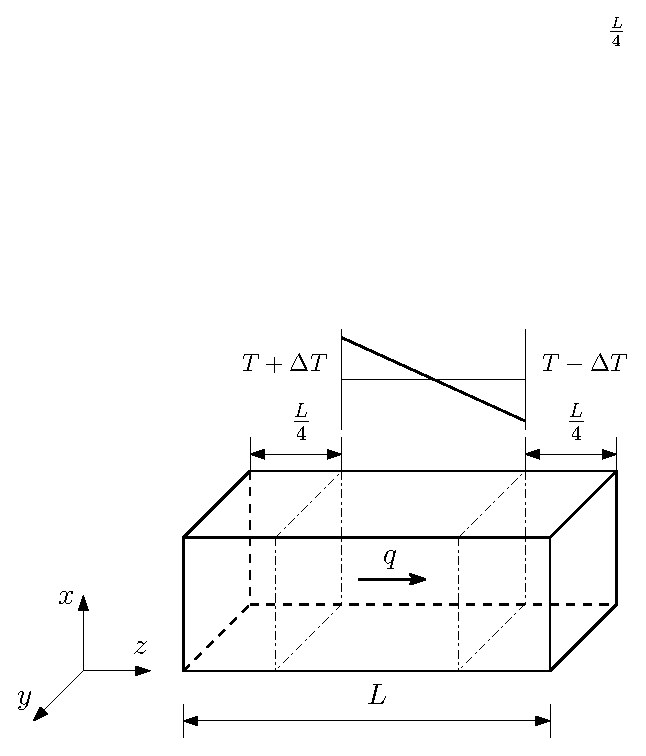
\includegraphics[width=0.48\textwidth]{./Figures/schematic}
%  &
%  \hspace{3mm}
%  \includegraphics[width=0.40\textwidth]{./Figures/Sibar_05}
%  \\ (a) & (b)
%  \end{tabular}
%\caption{(a) Schematic illustration of the set-up for evaluating thermal conductivity of Si using NEMD. (b) 
%Arrangement of Si atoms prior to the application of thermal gradient.}
%\label{fig:setup}
%\end{center}
%\end{figure}
%
%\clearpage

%%%%%%%%%%%%%%%%%%%%%%%%%%%%%%%%%%%%%%%%%%%%%%%%%%%%%%%%%%%%%%%%%%%%%%%%%

%\begin{figure}[p]
% \begin{center}
%  \includegraphics[width=0.70\textwidth]{./Figures/temp_plot}
%\caption{Temperature distribution along a Si bar of length 14.74~nm for different scenarios of applied 
%thermal gradient.}
%\label{fig:kapitza}
%\end{center}
%\end{figure}
%
%
%\clearpage

%%%%%%%%%%%%%%%%%%%%%%%%%%%%%%%%%%%%%%%%%%%%%%%%%%%%%%%%%%%%%%%%%%%%%%%%%

%\begin{figure}[p]
%\begin{center}
%\begin{tabular}{cc}
%  \hspace{-12mm}
%  \includegraphics[width=0.60\textwidth]{./Figures/realz_quad300K}
%  &
%  \hspace{-9mm}
%  \includegraphics[width=0.56\textwidth]{./Figures/PCspectrum_300}
%  \\ (a) & (b)
%  \end{tabular}
%\caption{(a) Realizations of discrepancy in bulk thermal conductivity at the Gauss-Legendre quadrature notes are
%depicted using circles. The size of the circle in each case is proportional to the discrepancy estimate, also provided
% in cases where it is observed to be relatively large. (b) Spectrum of PC coefficients is depicted using circles of
% varying sizes, proportional to the log value of their magnitude. The computations were performed at 300 K.}
%\label{fig:rs1}
%\end{center}
%\end{figure}
%
%\clearpage
%
%%%%%%%%%%%%%%%%%%%%%%%%%%%%%%%%%%%%%%%%%%%%%%%%%%%%%%%%%%%%%%%%%%%%%%%%%%
%
%\begin{figure}[p]
%\begin{center}
%\begin{tabular}{cc}
% \hspace{-10mm}
%  \includegraphics[width=0.55\textwidth]{./Figures/err2D_300}
%  &
%  %\hspace{-9mm}
%  \includegraphics[width=0.55\textwidth]{./Figures/err2D_500}
%  \\ (a) & (b)
%  \end{tabular}
%  \\ \vspace{1mm}
%  \includegraphics[width=0.50\textwidth]{./Figures/err2D_s}
%  \\ (c)
%\caption{Response surface of the discrepancy in bulk thermal conductivity at (a) $T$ = 300~K and
% (b) $T$ = 500~K. Gauss-Legendre quadrature nodes are highlighted in both cases. (c) Sobol samples
% in the 2D domain used for verifying the accuracy of the response surfaces.}
%\label{fig:rs2}
%\end{center}
%\end{figure}
%
%\clearpage

%%%%%%%%%%%%%%%%%%%%%%%%%%%%%%%%%%%%%%%%%%%%%%%%%%%%%%%%%%%%%%%%%%%%%%%%%

%\begin{figure}[p]
%\begin{center}
%\begin{tabular}{cc}
% \hspace{-10mm}
%  \includegraphics[width=0.50\textwidth]{./Figures/kinv_300}
%  &
%  %\hspace{-9mm}
%  \includegraphics[width=0.50\textwidth]{./Figures/kinv_500}
%  \\ (a) & (b)
%  \end{tabular}
% \caption{Inverse of the bulk thermal conductivity estimates are plotted against the inverse of Si bar length
% using predictions from NEMD as well as estimates from the response surface at (a)  $T$ = 300~K and 
% (b) $T$ = 500~K.}
%\label{fig:rs3}
%\end{center}
%\end{figure}
%
%\clearpage

%%%%%%%%%%%%%%%%%%%%%%%%%%%%%%%%%%%%%%%%%%%%%%%%%%%%%%%%%%%%%%%%%%%%%%%%%
 
%\begin{figure}[p]
%\begin{center}
%\begin{tabular}{cc}
%  \includegraphics[width=0.40\textwidth]{./Figures/unstable}
%  &
%  \hspace{3mm}
%  \includegraphics[width=0.50\textwidth]{./Figures/lx_npt}
%  \\ (a) & (b)
%  \end{tabular}
%\caption{(a) A snapshot of the arrangement of atoms illustrating loss of
%structural integrity of the Si bar. 
%(b) Si bar length is plotted against the number of time steps during
%the NPT ensemble stage of the simulation.}
%\label{fig:dgsm1}
%\end{center}
%\end{figure}
%
%\clearpage

%%%%%%%%%%%%%%%%%%%%%%%%%%%%%%%%%%%%%%%%%%%%%%%%%%%%%%%%%%%%%%%%%%%%%%%%%

%\begin{figure}[p]
% \begin{center}
%  \includegraphics[width=0.70\textwidth]{./Figures/ub}
%\caption{The quantity $\hat{\mathcal{C}_i\mu_i}$ as computed after 4 iterations and data at 25(7+1)
%points is plotted for each SW potential parameter.}
%\label{fig:ub}
%\end{center}
%\end{figure}
%
%\clearpage


%%%%%%%%%%%%%%%%%%%%%%%%%%%%%%%%%%%%%%%%%%%%%%%%%%%%%%%%%%%%%%%%%%%%%%%%%

%\begin{figure}[p]
% \begin{center}
%  \includegraphics[width=0.70\textwidth]{./Figures/PCE5D_eloo}
%\caption{A convergence study for the 5D PCE wherein the leave-one-out
%error, $\epsilon_{\tiny{\mbox{LOO}}}$ is plotted against the number of
%realizations or NEMD runs used to estimate the PC coefficients.}
%\label{fig:loo}
%\end{center}
%\end{figure}
%
%\clearpage

%%%%%%%%%%%%%%%%%%%%%%%%%%%%%%%%%%%%%%%%%%%%%%%%%%%%%%%%%%%%%%%%%%%%%%%%%

%\begin{figure}[p]
% \begin{center}
%  \includegraphics[width=0.70\textwidth]{./Figures/PCE5D_kde}
%\caption{Comparison of bulk thermal conductivity ($\kappa$) distribution of Si based on a histogram plot
%using NEMD predictions (Model) at 25 points in the 7D parameter space and a probability distribution obtained 
%using kernel density estimation of  reduced order surrogate estimates of $\kappa$ for 10$^6$ samples in the 5D
%parameter space.}
%\label{fig:verify}
%\end{center}
%\end{figure}
%
%\clearpage

%%%%%%%%%%%%%%%%%%%%%%%%%%%%%%%%%%%%%%%%%%%%%%%%%%%%%%%%%%%%%%%%%%%%%%%%%

%\begin{figure}[p]
% \begin{center}
%  \includegraphics[width=0.70\textwidth]{./Figures/PCE5D_gsa}
%\caption{Sobol first-order and total effect sensitivity indices as obtained using the reduced order PC
%surrogate and 10$^{6}$ samples in the 5D parameter space. }
%\label{fig:gsa}
%\end{center}
%\end{figure}
%
%\clearpage

%%%%%%%%%%%%%%%%%%%%%%%%%%%%%%%%%%%%%%%%%%%%%%%%%%%%%%%%%%%%%%%%%%%%%%%%%

%\begin{figure}[p]
% \begin{center}
%  \includegraphics[width=0.70\textwidth]{./Figures/gl}
%  \\ (a)
%  \begin{tabular}{cc}
%  \includegraphics[width=0.50\textwidth]{./Figures/pdf_alpha}
%  &
%  %\hspace{3mm}
%  \includegraphics[width=0.50\textwidth]{./Figures/pdf_gamma}
%  \\ (b) & (c)
%  \end{tabular}
%\caption{(a) A joint likelihood as estimated using Eq.~\ref{eq:like} is plotted on a 2D cartesian grid
% ($\alpha\times\gamma$). Point corresponding to the maximum likelihood (MLE) is also highlighted.
% The likelihood is plotted along a line passing through MLE and parallel to the $\alpha$-axis
% in (b), and $\gamma$-axis in (c).}
%\label{fig:like}
%\end{center}
%\end{figure}
%
%\clearpage




%%%%%%%%%%%%%%%%%%%%%%%%%%%%%%%%%%%%%%%%%%%%%%%%%%%%%%%%%%%%%%%%%%%%%%%%%



%\clearpage

\end{document}
